\subsection{Introduction}

Searching for a static or moving target in a planar environment is a classic 
problem in robotics \cite{guibas1999visibility, suzuki1992searching, lavalle2000algorithm, stiffler2017persistent, kolling2007graph}. 
%
The setting applies to many real-world applications, including searching for
lost person/object, checking for potential hazards, and generally, search and rescue tasks conducted in a known environment. 
%
Research tackling this problem mostly focuses on devising a search plan with
different types of objectives, such as minimizing the total length of the
frontier of the search schedule from the start to the end 
\cite{kolling2017coordinated}, minimizing the number of robots used for 
the search plan in a visibility-based robot sensing model
\cite{megiddo1988complexity}, and so on.

In certain cases, the high-level plan for searching a given region may already be pre-determined and fixed. For example, in search and rescue efforts, a frequently carried out plan is to perform a single sweep of an environment with a marching frontier, which is easy to execute when many participating robots/agents are involved.
%
The high-level search plan may also be determined by existing algorithms that 
compute only the search frontier.
%
However, even in the case where the search plan consists of pre-determined 
sweep (frontier) lines; it remains non-trivial to find an optimal organization 
of the mobile robots to execute the search plan, for either minimizing the 
number of robots needed for a given sensing probability requirement or utilizing 
a fixed number of robots to maximize the minimum sensing probability of locating something in the environment. 

\begin{figure}[t]
\vspace{1.5mm}
    \centering

    \begin{subfigure}[t]{0.7\textwidth}
         \centering
        % \vspace{2.5mm}
         \includegraphics[width=\textwidth]{chapters/sc/fig/instance_2-eps-converted-to.pdf}
        %  \vspace{0.5mm}
         \caption{Optimal robot allocations in a vertical sweep}
         \label{fig:sc-vertical}
     \end{subfigure}
    
    %\includegraphics[width=.475\textwidth]{fig/instance_2-eps-converted-to.pdf}
    \medskip
    
    \begin{subfigure}[t]{0.4\textwidth}
         \centering
        % \vspace{2.5mm}
         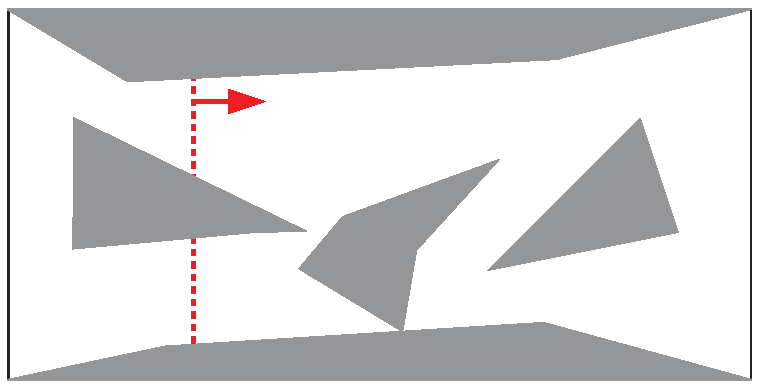
\includegraphics[width=\textwidth]{chapters/sc/fig/vertical-eps-converted-to.pdf}
        %  \vspace{0.5mm}
         \caption{Vertical}
         \label{fig:sc-vertical}
     \end{subfigure}
    \begin{subfigure}[t]{0.2\textwidth}
         \centering
         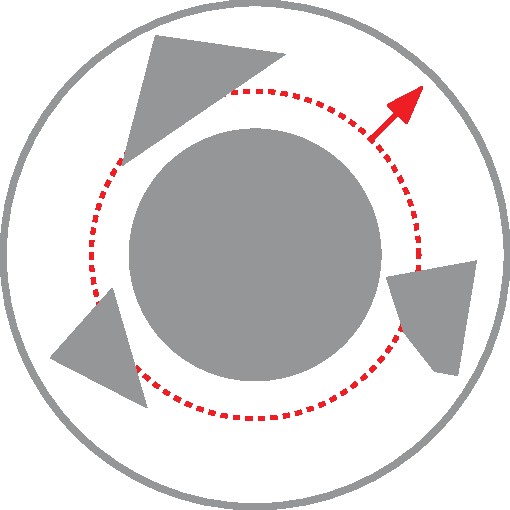
\includegraphics[width=\textwidth]{chapters/sc/fig/circular-eps-converted-to.pdf}
         \caption{Circular}
         \label{fig:sc-radial}
     \end{subfigure}
    \begin{subfigure}[t]{0.2\textwidth}
         \centering
         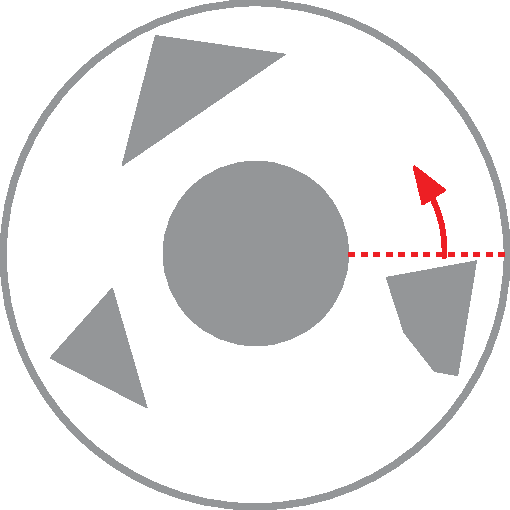
\includegraphics[width=\textwidth]{chapters/sc/fig/rotational-eps-converted-to.pdf}
         \caption{Radial}
         \label{fig:sc-circular}
    \end{subfigure}
     
    \vspace{2mm}
    \caption[Illustration of sweep schedules]{(a) An illustration of robots' locations along a left-to-right 
    vertical sweep schedule. Four robots are allocated to execute the vertical sweep, 
    and their trajectories are illustrated in different colors. 
    %
    % There exist discontinuities (jumps) along the trajectories when obstacle vertices 
    % intersect the sweep line, induced by topological changes of the environment. 
    (b)(c)(d) Illustrations of three use cases: vertical, circular, 
    and radial sweeps.}
    \label{fig:sc-sweep}
\end{figure}

In this work, we address the challenge of how to best allocate 
many robots to execute a pre-determined search schedule for a known environment. 
More specifically, for a two-dimensional closed and bounded workspace, and a known 
search schedule, which gives a search frontier for any given time, the robot guards 
are required to stay on the search frontier to carry out the sensing task. 
%
Because each robot's coverage quality deteriorates with distance, their relative 
placement on the frontier must be carefully decided to maximize the coverage quality. 
%
For the setup, we focus on the problem of finding the minimum number of robots required 
to execute a pre-determined sweep schedule such that a minimum sensing quality is 
guaranteed for each point in the workspace. Solutions to this minimization problem 
readily translate to solutions for maximizing the coverage quality for a fixed number 
of robots, which is a dual problem. 

In summary, the main contributions of this work are twofold. First, we generalize the 
notion of boustrophedon decomposition \cite{choset2000coverage}, which partitions the 
plane via vertical sweep, into a decomposition of the plane with a \emph{continuous 
monotone sweep schedule}, which we prove can always be represented as a directed 
acyclic graph (DAG). 
%
Then, we show the problem of minimizing the number of line guards required to execute a sweep schedule can be transformed into a network flow problem.
%
Since the generalized boustrophedon decomposition and the network flow problem can 
be solved in low polynomial time; our method achieves high levels of scalability.
%
The strengths of our method are further corroborated in extensive simulation experiments 
on three realistic use cases: \emph{vertical sweep}, \emph{circular sweep}, and 
\emph{radial sweep} (see, e.g., ~\ref{fig:sc-sweep} (b)(c)(d)).





\noindent
% \textbf{Related Work.}
% The study in this paper draws inspiration from the study of several 
% lines of related problems. 
% The Graph-Clear problem, formulated in \cite{kolling2007graph}, tasks a group of robots to search and clear an environment with the operations of blocking and clearing.
% A follow-up work on Line-Clear \cite{kolling2017coordinated} uses line guards
% with more focus on computational geometry in that
% the objective is to minimize the maximum sweep line distance. Both of these problems are
% NP-hard, establishing the difficulties of finding a sweep schedule for a planar environment.
% The more general pursuit-evasion problem dates back to the research on \emph{search number}
% on a discrete graph \cite{megiddo1988complexity}, 
% followed by studies on pursuit and evasion continuous environment with 
% visibility-based model \cite{guibas1999visibility, suzuki1992searching, lavalle2000algorithm, stiffler2017persistent}. 
% The problem becomes the well-known art-gallery problem \cite{o1987art} when a static deployment of robots is sought after.
%
% When working with known patrolling search frontiers, e.g., vertical sweep lines, 
% this problem is analogous to the perimeter defense problem by placing guards on a static perimeter
% to defend intruders \cite{shishika2020cooperative, macharet2020adaptive, chen2021optimal}.
% Previously, we have also studied a version of static range guard placement problems for securing perimeters and regions \cite{fengyu2020optimally}.
% In contrast to the pursuit-evasion algorithms that deal with searching dynamic and unpredictable targets that could escape, 
% coverage planning/control-related algorithms become more suitable for searching or covering predictable or stationary targets,
% e.g., room sweeping, pesticide and fertilizer spraying, persistent monitoring, and so on \cite{cortes2004coverage, oksanen2009coverage, haksar2020spatial, wei2018coverage, deng2019constrained, lan2013planning, cassandras2012optimal, yu2015persistent, palacios2017optimal}. 

\begin{comment}
\noindent
\textbf{Search and rescue}
Graph Clear / Line Clear: 
Andreas Kolling's work like his thesis and some following work as "Coordinated search with multiple robots arranged in line formations" 

\noindent
\textbf{Pursuit evasion}
\noindent
Visibility based: ...

\noindent
\textbf{perimeter defense/guarding}

\noindent
\textbf{Coverage planning}: 
Similar vertical (trapezoidal, boustrophedon) tessellation of plane 

\noindent
"Coverage of Known Spaces: The Boustrophedon Cellular Decomposition"

\noindent
"On Minimizing Turns in Robot Coverage Path Planning"

\noindent
"Coverage Path Planning Algorithms for Agricultural Field Machines"

\noindent
"Optimal Line-sweep-based Decompositions for Coverage Algorithms"



\end{comment}
